\documentclass[twoside]{book}

% Packages required by doxygen
\usepackage{fixltx2e}
\usepackage{calc}
\usepackage{doxygen}
\usepackage[export]{adjustbox} % also loads graphicx
\usepackage{graphicx}
\usepackage[utf8]{inputenc}
\usepackage{makeidx}
\usepackage{multicol}
\usepackage{multirow}
\PassOptionsToPackage{warn}{textcomp}
\usepackage{textcomp}
\usepackage[nointegrals]{wasysym}
\usepackage[table]{xcolor}

% Font selection
\usepackage[T1]{fontenc}
\usepackage[scaled=.90]{helvet}
\usepackage{courier}
\usepackage{amssymb}
\usepackage{sectsty}
\renewcommand{\familydefault}{\sfdefault}
\allsectionsfont{%
  \fontseries{bc}\selectfont%
  \color{darkgray}%
}
\renewcommand{\DoxyLabelFont}{%
  \fontseries{bc}\selectfont%
  \color{darkgray}%
}
\newcommand{\+}{\discretionary{\mbox{\scriptsize$\hookleftarrow$}}{}{}}

% Page & text layout
\usepackage{geometry}
\geometry{%
  a4paper,%
  top=2.5cm,%
  bottom=2.5cm,%
  left=2.5cm,%
  right=2.5cm%
}
\tolerance=750
\hfuzz=15pt
\hbadness=750
\setlength{\emergencystretch}{15pt}
\setlength{\parindent}{0cm}
\setlength{\parskip}{3ex plus 2ex minus 2ex}
\makeatletter
\renewcommand{\paragraph}{%
  \@startsection{paragraph}{4}{0ex}{-1.0ex}{1.0ex}{%
    \normalfont\normalsize\bfseries\SS@parafont%
  }%
}
\renewcommand{\subparagraph}{%
  \@startsection{subparagraph}{5}{0ex}{-1.0ex}{1.0ex}{%
    \normalfont\normalsize\bfseries\SS@subparafont%
  }%
}
\makeatother

% Headers & footers
\usepackage{fancyhdr}
\pagestyle{fancyplain}
\fancyhead[LE]{\fancyplain{}{\bfseries\thepage}}
\fancyhead[CE]{\fancyplain{}{}}
\fancyhead[RE]{\fancyplain{}{\bfseries\leftmark}}
\fancyhead[LO]{\fancyplain{}{\bfseries\rightmark}}
\fancyhead[CO]{\fancyplain{}{}}
\fancyhead[RO]{\fancyplain{}{\bfseries\thepage}}
\fancyfoot[LE]{\fancyplain{}{}}
\fancyfoot[CE]{\fancyplain{}{}}
\fancyfoot[RE]{\fancyplain{}{\bfseries\scriptsize Generated by Doxygen }}
\fancyfoot[LO]{\fancyplain{}{\bfseries\scriptsize Generated by Doxygen }}
\fancyfoot[CO]{\fancyplain{}{}}
\fancyfoot[RO]{\fancyplain{}{}}
\renewcommand{\footrulewidth}{0.4pt}
\renewcommand{\chaptermark}[1]{%
  \markboth{#1}{}%
}
\renewcommand{\sectionmark}[1]{%
  \markright{\thesection\ #1}%
}

% Indices & bibliography
\usepackage{natbib}
\usepackage[titles]{tocloft}
\setcounter{tocdepth}{3}
\setcounter{secnumdepth}{5}
\makeindex

% Hyperlinks (required, but should be loaded last)
\usepackage{ifpdf}
\ifpdf
  \usepackage[pdftex,pagebackref=true]{hyperref}
\else
  \usepackage[ps2pdf,pagebackref=true]{hyperref}
\fi
\hypersetup{%
  colorlinks=true,%
  linkcolor=blue,%
  citecolor=blue,%
  unicode%
}

% Custom commands
\newcommand{\clearemptydoublepage}{%
  \newpage{\pagestyle{empty}\cleardoublepage}%
}

\usepackage{caption}
\captionsetup{labelsep=space,justification=centering,font={bf},singlelinecheck=off,skip=4pt,position=top}

%===== C O N T E N T S =====

\begin{document}

% Titlepage & ToC
\hypersetup{pageanchor=false,
             bookmarksnumbered=true,
             pdfencoding=unicode
            }
\pagenumbering{roman}
\begin{titlepage}
\vspace*{7cm}
\begin{center}%
{\Large M\+S\+S\+P\+M\+\_\+\+Gui\+Estimation }\\
\vspace*{1cm}
{\large Generated by Doxygen 1.8.11}\\
\end{center}
\end{titlepage}
\clearemptydoublepage
\tableofcontents
\clearemptydoublepage
\pagenumbering{arabic}
\hypersetup{pageanchor=true}

%--- Begin generated contents ---
\chapter{Hierarchical Index}
\section{Class Hierarchy}
This inheritance list is sorted roughly, but not completely, alphabetically\+:\begin{DoxyCompactList}
\item Q\+Object\begin{DoxyCompactList}
\item \contentsline{section}{nmf\+Estimation\+\_\+\+Tab1}{\pageref{classnmf_estimation___tab1}}{}
\item \contentsline{section}{nmf\+Estimation\+\_\+\+Tab2}{\pageref{classnmf_estimation___tab2}}{}
\item \contentsline{section}{nmf\+Estimation\+\_\+\+Tab3}{\pageref{classnmf_estimation___tab3}}{}
\item \contentsline{section}{nmf\+Estimation\+\_\+\+Tab4}{\pageref{classnmf_estimation___tab4}}{}
\item \contentsline{section}{nmf\+Estimation\+\_\+\+Tab5}{\pageref{classnmf_estimation___tab5}}{}
\item \contentsline{section}{nmf\+Estimation\+\_\+\+Tab6}{\pageref{classnmf_estimation___tab6}}{}
\end{DoxyCompactList}
\end{DoxyCompactList}

\chapter{Class Index}
\section{Class List}
Here are the classes, structs, unions and interfaces with brief descriptions\+:\begin{DoxyCompactList}
\item\contentsline{section}{\hyperlink{classnmf_estimation___tab1}{nmf\+Estimation\+\_\+\+Tab1} \\*Estimated Parameters }{\pageref{classnmf_estimation___tab1}}{}
\item\contentsline{section}{\hyperlink{classnmf_estimation___tab2}{nmf\+Estimation\+\_\+\+Tab2} \\*Catch data }{\pageref{classnmf_estimation___tab2}}{}
\item\contentsline{section}{\hyperlink{classnmf_estimation___tab3}{nmf\+Estimation\+\_\+\+Tab3} \\*Competition Tables }{\pageref{classnmf_estimation___tab3}}{}
\item\contentsline{section}{\hyperlink{classnmf_estimation___tab4}{nmf\+Estimation\+\_\+\+Tab4} \\*Predation Tables }{\pageref{classnmf_estimation___tab4}}{}
\item\contentsline{section}{\hyperlink{classnmf_estimation___tab5}{nmf\+Estimation\+\_\+\+Tab5} \\*Biomass Table }{\pageref{classnmf_estimation___tab5}}{}
\item\contentsline{section}{\hyperlink{classnmf_estimation___tab6}{nmf\+Estimation\+\_\+\+Tab6} \\*The Run Estimation Settings }{\pageref{classnmf_estimation___tab6}}{}
\end{DoxyCompactList}

\chapter{Class Documentation}
\hypertarget{classnmf_estimation___tab1}{}\section{nmf\+Estimation\+\_\+\+Tab1 Class Reference}
\label{classnmf_estimation___tab1}\index{nmf\+Estimation\+\_\+\+Tab1@{nmf\+Estimation\+\_\+\+Tab1}}


Estimated Parameters.  




{\ttfamily \#include $<$nmf\+Estimation\+Tab01.\+h$>$}



Inheritance diagram for nmf\+Estimation\+\_\+\+Tab1\+:\nopagebreak
\begin{figure}[H]
\begin{center}
\leavevmode
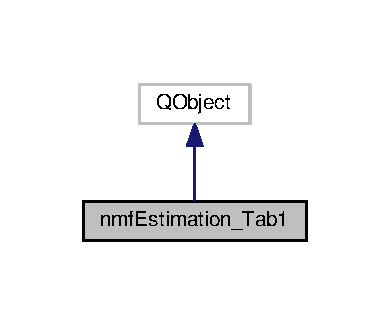
\includegraphics[width=187pt]{classnmf_estimation___tab1__inherit__graph}
\end{center}
\end{figure}


Collaboration diagram for nmf\+Estimation\+\_\+\+Tab1\+:\nopagebreak
\begin{figure}[H]
\begin{center}
\leavevmode
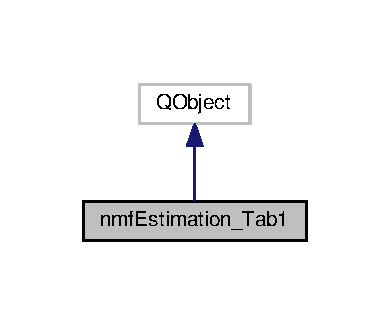
\includegraphics[width=187pt]{classnmf_estimation___tab1__coll__graph}
\end{center}
\end{figure}
\subsection*{Public Slots}
\begin{DoxyCompactItemize}
\item 
void {\bfseries callback\+\_\+\+Load\+PB} ()\hypertarget{classnmf_estimation___tab1_a111a517b2d9892c2762a13b512d9f3f7}{}\label{classnmf_estimation___tab1_a111a517b2d9892c2762a13b512d9f3f7}

\item 
void {\bfseries callback\+\_\+\+Save\+PB} ()\hypertarget{classnmf_estimation___tab1_a9741486fd83c5ed7000ef9887e5ef947}{}\label{classnmf_estimation___tab1_a9741486fd83c5ed7000ef9887e5ef947}

\item 
void {\bfseries callback\+\_\+\+Next\+PB} ()\hypertarget{classnmf_estimation___tab1_a2228ff0a3b9ec7b484b37a515baab971}{}\label{classnmf_estimation___tab1_a2228ff0a3b9ec7b484b37a515baab971}

\end{DoxyCompactItemize}
\subsection*{Signals}
\begin{DoxyCompactItemize}
\item 
void {\bfseries Reload\+Species} ()\hypertarget{classnmf_estimation___tab1_adbc14781521eb3f593b62e5f010d6517}{}\label{classnmf_estimation___tab1_adbc14781521eb3f593b62e5f010d6517}

\end{DoxyCompactItemize}
\subsection*{Public Member Functions}
\begin{DoxyCompactItemize}
\item 
\hyperlink{classnmf_estimation___tab1_ac5bfc5f07973b3cff7f34a1c2fe443fd}{nmf\+Estimation\+\_\+\+Tab1} (Q\+Tab\+Widget $\ast$tabs, nmf\+Logger $\ast$logger, nmf\+Database $\ast$database\+Ptr, std\+::string \&project\+Dir)
\begin{DoxyCompactList}\small\item\em \hyperlink{classnmf_estimation___tab1}{nmf\+Estimation\+\_\+\+Tab1} \+: class constructor \end{DoxyCompactList}\item 
bool {\bfseries load\+Widgets} ()\hypertarget{classnmf_estimation___tab1_a90da30669095e091b7057696bc1b72b4}{}\label{classnmf_estimation___tab1_a90da30669095e091b7057696bc1b72b4}

\item 
void {\bfseries clear\+Widgets} ()\hypertarget{classnmf_estimation___tab1_a0e41a91dbc55562ba02fb9eef37a35e6}{}\label{classnmf_estimation___tab1_a0e41a91dbc55562ba02fb9eef37a35e6}

\end{DoxyCompactItemize}


\subsection{Detailed Description}
Estimated Parameters. 

This table is reproduced here from the Species table in Setup Tab 3. This is a more succinct way of looking at the per Species estimated parameters and their min/max values. 

\subsection{Constructor \& Destructor Documentation}
\index{nmf\+Estimation\+\_\+\+Tab1@{nmf\+Estimation\+\_\+\+Tab1}!nmf\+Estimation\+\_\+\+Tab1@{nmf\+Estimation\+\_\+\+Tab1}}
\index{nmf\+Estimation\+\_\+\+Tab1@{nmf\+Estimation\+\_\+\+Tab1}!nmf\+Estimation\+\_\+\+Tab1@{nmf\+Estimation\+\_\+\+Tab1}}
\subsubsection[{\texorpdfstring{nmf\+Estimation\+\_\+\+Tab1(\+Q\+Tab\+Widget $\ast$tabs, nmf\+Logger $\ast$logger, nmf\+Database $\ast$database\+Ptr, std\+::string \&project\+Dir)}{nmfEstimation_Tab1(QTabWidget *tabs, nmfLogger *logger, nmfDatabase *databasePtr, std::string &projectDir)}}]{\setlength{\rightskip}{0pt plus 5cm}nmf\+Estimation\+\_\+\+Tab1\+::nmf\+Estimation\+\_\+\+Tab1 (
\begin{DoxyParamCaption}
\item[{Q\+Tab\+Widget $\ast$}]{tabs, }
\item[{nmf\+Logger $\ast$}]{logger, }
\item[{nmf\+Database $\ast$}]{database\+Ptr, }
\item[{std\+::string \&}]{project\+Dir}
\end{DoxyParamCaption}
)}\hypertarget{classnmf_estimation___tab1_ac5bfc5f07973b3cff7f34a1c2fe443fd}{}\label{classnmf_estimation___tab1_ac5bfc5f07973b3cff7f34a1c2fe443fd}


\hyperlink{classnmf_estimation___tab1}{nmf\+Estimation\+\_\+\+Tab1} \+: class constructor 


\begin{DoxyParams}{Parameters}
{\em tabs} & \+: the tab widget into which this Estimation tab will be placed \\
\hline
{\em logger} & \+: pointer to the application logger \\
\hline
{\em database\+Ptr} & \+: pointer to the application database \\
\hline
{\em project\+Dir} & \+: the project directory \\
\hline
\end{DoxyParams}


The documentation for this class was generated from the following files\+:\begin{DoxyCompactItemize}
\item 
nmf\+Estimation\+Tab01.\+h\item 
nmf\+Estimation\+Tab01.\+cpp\end{DoxyCompactItemize}

\hypertarget{classnmf_estimation___tab2}{}\section{nmf\+Estimation\+\_\+\+Tab2 Class Reference}
\label{classnmf_estimation___tab2}\index{nmf\+Estimation\+\_\+\+Tab2@{nmf\+Estimation\+\_\+\+Tab2}}


Catch data.  




{\ttfamily \#include $<$nmf\+Estimation\+Tab02.\+h$>$}



Inheritance diagram for nmf\+Estimation\+\_\+\+Tab2\+:\nopagebreak
\begin{figure}[H]
\begin{center}
\leavevmode
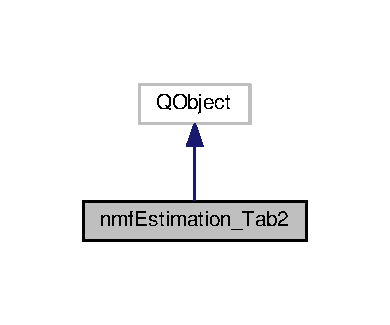
\includegraphics[width=187pt]{classnmf_estimation___tab2__inherit__graph}
\end{center}
\end{figure}


Collaboration diagram for nmf\+Estimation\+\_\+\+Tab2\+:\nopagebreak
\begin{figure}[H]
\begin{center}
\leavevmode
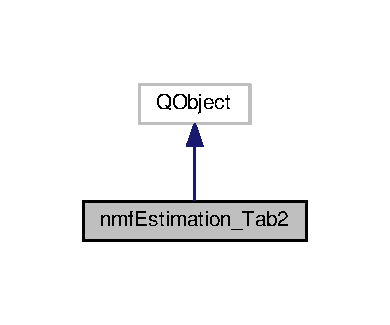
\includegraphics[width=187pt]{classnmf_estimation___tab2__coll__graph}
\end{center}
\end{figure}
\subsection*{Public Slots}
\begin{DoxyCompactItemize}
\item 
void {\bfseries callback\+\_\+\+Load\+PB} ()\hypertarget{classnmf_estimation___tab2_a4f081c9228c16d7bfc430c719bab9fea}{}\label{classnmf_estimation___tab2_a4f081c9228c16d7bfc430c719bab9fea}

\item 
void {\bfseries callback\+\_\+\+Save\+PB} ()\hypertarget{classnmf_estimation___tab2_aaae777a753a648698472f1b80a0ee84a}{}\label{classnmf_estimation___tab2_aaae777a753a648698472f1b80a0ee84a}

\item 
void {\bfseries callback\+\_\+\+Prev\+PB} ()\hypertarget{classnmf_estimation___tab2_ae41c2f59eb16add1033d18bfce26b5ba}{}\label{classnmf_estimation___tab2_ae41c2f59eb16add1033d18bfce26b5ba}

\item 
void {\bfseries callback\+\_\+\+Next\+PB} ()\hypertarget{classnmf_estimation___tab2_a4ddbed0f122af965a66316e1994523b5}{}\label{classnmf_estimation___tab2_a4ddbed0f122af965a66316e1994523b5}

\item 
void {\bfseries callback\+\_\+\+Harvest\+Form\+Changed} (Q\+String harvest\+Form)\hypertarget{classnmf_estimation___tab2_a330174fcdd6956c61cf25b013eb7fa6d}{}\label{classnmf_estimation___tab2_a330174fcdd6956c61cf25b013eb7fa6d}

\end{DoxyCompactItemize}
\subsection*{Public Member Functions}
\begin{DoxyCompactItemize}
\item 
\hyperlink{classnmf_estimation___tab2_a81c4d112cfb52709ba46a2c287ea426e}{nmf\+Estimation\+\_\+\+Tab2} (Q\+Tab\+Widget $\ast$tabs, nmf\+Logger $\ast$logger, nmf\+Database $\ast$database\+Ptr, std\+::string \&project\+Dir)
\begin{DoxyCompactList}\small\item\em \hyperlink{classnmf_estimation___tab2}{nmf\+Estimation\+\_\+\+Tab2} \+: class constructor \end{DoxyCompactList}\item 
bool {\bfseries load\+Widgets} ()\hypertarget{classnmf_estimation___tab2_aa8b3ddbb2db6ff90cb2048bf4f87506e}{}\label{classnmf_estimation___tab2_aa8b3ddbb2db6ff90cb2048bf4f87506e}

\item 
bool {\bfseries load\+Widgets} (Q\+String Mohns\+Rho\+Label)\hypertarget{classnmf_estimation___tab2_a6d872df42e5a0bb847897fb36fa26766}{}\label{classnmf_estimation___tab2_a6d872df42e5a0bb847897fb36fa26766}

\item 
void {\bfseries clear\+Widgets} ()\hypertarget{classnmf_estimation___tab2_aa28f54f7a7c2cf18d31ca7df6e46d781}{}\label{classnmf_estimation___tab2_aa28f54f7a7c2cf18d31ca7df6e46d781}

\item 
void {\bfseries read\+Settings} ()\hypertarget{classnmf_estimation___tab2_a7dc05290661a758d33ba3b4f0cb4209d}{}\label{classnmf_estimation___tab2_a7dc05290661a758d33ba3b4f0cb4209d}

\item 
void {\bfseries set\+Harvest\+Type} (std\+::string harvest\+Type)\hypertarget{classnmf_estimation___tab2_a61801ee8195b5c9eb71750d71d8fb903}{}\label{classnmf_estimation___tab2_a61801ee8195b5c9eb71750d71d8fb903}

\end{DoxyCompactItemize}


\subsection{Detailed Description}
Catch data. 

This table represents the Catch data for the year range and for each Species. The user should save newly modified Catch data prior to progressing to the next tab. 

\subsection{Constructor \& Destructor Documentation}
\index{nmf\+Estimation\+\_\+\+Tab2@{nmf\+Estimation\+\_\+\+Tab2}!nmf\+Estimation\+\_\+\+Tab2@{nmf\+Estimation\+\_\+\+Tab2}}
\index{nmf\+Estimation\+\_\+\+Tab2@{nmf\+Estimation\+\_\+\+Tab2}!nmf\+Estimation\+\_\+\+Tab2@{nmf\+Estimation\+\_\+\+Tab2}}
\subsubsection[{\texorpdfstring{nmf\+Estimation\+\_\+\+Tab2(\+Q\+Tab\+Widget $\ast$tabs, nmf\+Logger $\ast$logger, nmf\+Database $\ast$database\+Ptr, std\+::string \&project\+Dir)}{nmfEstimation_Tab2(QTabWidget *tabs, nmfLogger *logger, nmfDatabase *databasePtr, std::string &projectDir)}}]{\setlength{\rightskip}{0pt plus 5cm}nmf\+Estimation\+\_\+\+Tab2\+::nmf\+Estimation\+\_\+\+Tab2 (
\begin{DoxyParamCaption}
\item[{Q\+Tab\+Widget $\ast$}]{tabs, }
\item[{nmf\+Logger $\ast$}]{logger, }
\item[{nmf\+Database $\ast$}]{database\+Ptr, }
\item[{std\+::string \&}]{project\+Dir}
\end{DoxyParamCaption}
)}\hypertarget{classnmf_estimation___tab2_a81c4d112cfb52709ba46a2c287ea426e}{}\label{classnmf_estimation___tab2_a81c4d112cfb52709ba46a2c287ea426e}


\hyperlink{classnmf_estimation___tab2}{nmf\+Estimation\+\_\+\+Tab2} \+: class constructor 


\begin{DoxyParams}{Parameters}
{\em tabs} & \+: the tab widget into which this Estimation tab will be placed \\
\hline
{\em logger} & \+: pointer to the application logger \\
\hline
{\em database\+Ptr} & \+: pointer to the application database \\
\hline
{\em project\+Dir} & \+: the project directory \\
\hline
\end{DoxyParams}


The documentation for this class was generated from the following files\+:\begin{DoxyCompactItemize}
\item 
nmf\+Estimation\+Tab02.\+h\item 
nmf\+Estimation\+Tab02.\+cpp\end{DoxyCompactItemize}

\hypertarget{classnmf_estimation___tab3}{}\section{nmf\+Estimation\+\_\+\+Tab3 Class Reference}
\label{classnmf_estimation___tab3}\index{nmf\+Estimation\+\_\+\+Tab3@{nmf\+Estimation\+\_\+\+Tab3}}


Competition Tables.  




{\ttfamily \#include $<$nmf\+Estimation\+Tab03.\+h$>$}



Inheritance diagram for nmf\+Estimation\+\_\+\+Tab3\+:\nopagebreak
\begin{figure}[H]
\begin{center}
\leavevmode
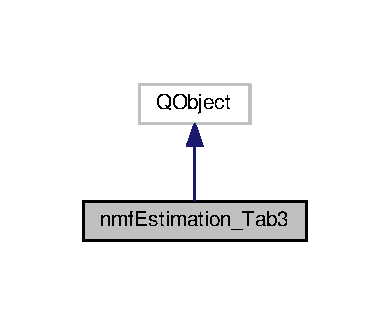
\includegraphics[width=187pt]{classnmf_estimation___tab3__inherit__graph}
\end{center}
\end{figure}


Collaboration diagram for nmf\+Estimation\+\_\+\+Tab3\+:\nopagebreak
\begin{figure}[H]
\begin{center}
\leavevmode
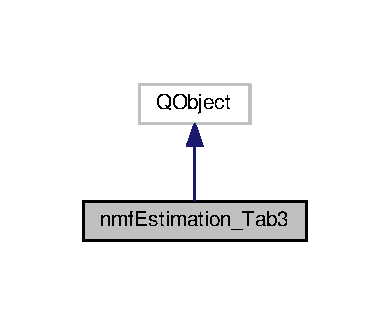
\includegraphics[width=187pt]{classnmf_estimation___tab3__coll__graph}
\end{center}
\end{figure}
\subsection*{Public Slots}
\begin{DoxyCompactItemize}
\item 
void {\bfseries callback\+\_\+\+Load\+PB} ()\hypertarget{classnmf_estimation___tab3_a576c64050facddb6c69e66900a37bf9b}{}\label{classnmf_estimation___tab3_a576c64050facddb6c69e66900a37bf9b}

\item 
void {\bfseries callback\+\_\+\+Save\+PB} ()\hypertarget{classnmf_estimation___tab3_a1e941f6d64899c4d6ebab2d1d968af95}{}\label{classnmf_estimation___tab3_a1e941f6d64899c4d6ebab2d1d968af95}

\item 
void {\bfseries callback\+\_\+\+Prev\+PB} ()\hypertarget{classnmf_estimation___tab3_a87f8f066b3eaf5c9029e574563e16ece}{}\label{classnmf_estimation___tab3_a87f8f066b3eaf5c9029e574563e16ece}

\item 
void {\bfseries callback\+\_\+\+Next\+PB} ()\hypertarget{classnmf_estimation___tab3_a1f24754398b1191bf71dce2ebb712700}{}\label{classnmf_estimation___tab3_a1f24754398b1191bf71dce2ebb712700}

\item 
void {\bfseries callback\+\_\+min\+Splitter\+Moved} (int pos, int index)\hypertarget{classnmf_estimation___tab3_ac8cba4aedbbda2501ea61de36b1daf68}{}\label{classnmf_estimation___tab3_ac8cba4aedbbda2501ea61de36b1daf68}

\item 
void {\bfseries callback\+\_\+max\+Splitter\+Moved} (int pos, int index)\hypertarget{classnmf_estimation___tab3_a59d5e1b5de967189037598d7bfb60022}{}\label{classnmf_estimation___tab3_a59d5e1b5de967189037598d7bfb60022}

\item 
void {\bfseries callback\+\_\+\+Competition\+Form\+Changed} (Q\+String competition\+Form)\hypertarget{classnmf_estimation___tab3_a10dfee72ed67b52afec72060531bfbb1}{}\label{classnmf_estimation___tab3_a10dfee72ed67b52afec72060531bfbb1}

\item 
void {\bfseries callback\+\_\+\+Estimate\+Checked} (int state)\hypertarget{classnmf_estimation___tab3_a42f31bad5e3e9377c671e6f58825c62f}{}\label{classnmf_estimation___tab3_a42f31bad5e3e9377c671e6f58825c62f}

\end{DoxyCompactItemize}
\subsection*{Public Member Functions}
\begin{DoxyCompactItemize}
\item 
\hyperlink{classnmf_estimation___tab3_a66d00a2486349efb1fc71f6e5a83f306}{nmf\+Estimation\+\_\+\+Tab3} (Q\+Tab\+Widget $\ast$tabs, nmf\+Logger $\ast$logger, nmf\+Database $\ast$database\+Ptr, std\+::string \&project\+Dir)
\begin{DoxyCompactList}\small\item\em \hyperlink{classnmf_estimation___tab3}{nmf\+Estimation\+\_\+\+Tab3} \+: class constructor \end{DoxyCompactList}\item 
bool {\bfseries load\+Widgets} ()\hypertarget{classnmf_estimation___tab3_ae5a06add9874cf6f04c5890090a500bc}{}\label{classnmf_estimation___tab3_ae5a06add9874cf6f04c5890090a500bc}

\item 
void {\bfseries clear\+Widgets} ()\hypertarget{classnmf_estimation___tab3_ac181a0f5624567062f2de767e3053b73}{}\label{classnmf_estimation___tab3_ac181a0f5624567062f2de767e3053b73}

\item 
void {\bfseries read\+Settings} ()\hypertarget{classnmf_estimation___tab3_a1c9101256d17a175fefefd3562a9cb8b}{}\label{classnmf_estimation___tab3_a1c9101256d17a175fefefd3562a9cb8b}

\item 
void {\bfseries get\+Algorithm} (std\+::string \&Algorithm)\hypertarget{classnmf_estimation___tab3_aa396e8a347ab98dd3c5029020cdac57e}{}\label{classnmf_estimation___tab3_aa396e8a347ab98dd3c5029020cdac57e}

\end{DoxyCompactItemize}


\subsection{Detailed Description}
Competition Tables. 

These tables allow user to enter and modify minimum and maximum alpha and beta food Competition data. 

\subsection{Constructor \& Destructor Documentation}
\index{nmf\+Estimation\+\_\+\+Tab3@{nmf\+Estimation\+\_\+\+Tab3}!nmf\+Estimation\+\_\+\+Tab3@{nmf\+Estimation\+\_\+\+Tab3}}
\index{nmf\+Estimation\+\_\+\+Tab3@{nmf\+Estimation\+\_\+\+Tab3}!nmf\+Estimation\+\_\+\+Tab3@{nmf\+Estimation\+\_\+\+Tab3}}
\subsubsection[{\texorpdfstring{nmf\+Estimation\+\_\+\+Tab3(\+Q\+Tab\+Widget $\ast$tabs, nmf\+Logger $\ast$logger, nmf\+Database $\ast$database\+Ptr, std\+::string \&project\+Dir)}{nmfEstimation_Tab3(QTabWidget *tabs, nmfLogger *logger, nmfDatabase *databasePtr, std::string &projectDir)}}]{\setlength{\rightskip}{0pt plus 5cm}nmf\+Estimation\+\_\+\+Tab3\+::nmf\+Estimation\+\_\+\+Tab3 (
\begin{DoxyParamCaption}
\item[{Q\+Tab\+Widget $\ast$}]{tabs, }
\item[{nmf\+Logger $\ast$}]{logger, }
\item[{nmf\+Database $\ast$}]{database\+Ptr, }
\item[{std\+::string \&}]{project\+Dir}
\end{DoxyParamCaption}
)}\hypertarget{classnmf_estimation___tab3_a66d00a2486349efb1fc71f6e5a83f306}{}\label{classnmf_estimation___tab3_a66d00a2486349efb1fc71f6e5a83f306}


\hyperlink{classnmf_estimation___tab3}{nmf\+Estimation\+\_\+\+Tab3} \+: class constructor 


\begin{DoxyParams}{Parameters}
{\em tabs} & \+: the tab widget into which this Estimation tab will be placed \\
\hline
{\em logger} & \+: pointer to the application logger \\
\hline
{\em database\+Ptr} & \+: pointer to the application database \\
\hline
{\em project\+Dir} & \+: the project directory \\
\hline
\end{DoxyParams}


The documentation for this class was generated from the following files\+:\begin{DoxyCompactItemize}
\item 
nmf\+Estimation\+Tab03.\+h\item 
nmf\+Estimation\+Tab03.\+cpp\end{DoxyCompactItemize}

\hypertarget{classnmf_estimation___tab4}{}\section{nmf\+Estimation\+\_\+\+Tab4 Class Reference}
\label{classnmf_estimation___tab4}\index{nmf\+Estimation\+\_\+\+Tab4@{nmf\+Estimation\+\_\+\+Tab4}}


Predation Tables.  




{\ttfamily \#include $<$nmf\+Estimation\+Tab04.\+h$>$}



Inheritance diagram for nmf\+Estimation\+\_\+\+Tab4\+:\nopagebreak
\begin{figure}[H]
\begin{center}
\leavevmode
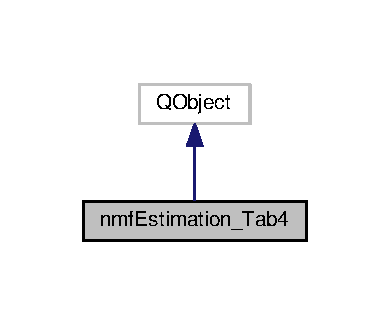
\includegraphics[width=187pt]{classnmf_estimation___tab4__inherit__graph}
\end{center}
\end{figure}


Collaboration diagram for nmf\+Estimation\+\_\+\+Tab4\+:\nopagebreak
\begin{figure}[H]
\begin{center}
\leavevmode
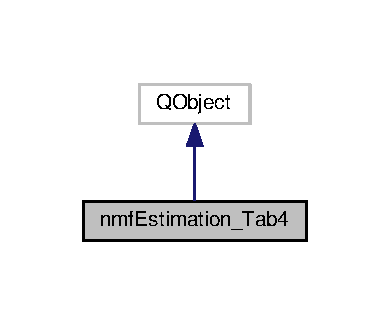
\includegraphics[width=187pt]{classnmf_estimation___tab4__coll__graph}
\end{center}
\end{figure}
\subsection*{Public Slots}
\begin{DoxyCompactItemize}
\item 
void {\bfseries callback\+\_\+\+Load\+PB} ()\hypertarget{classnmf_estimation___tab4_a3cb2313c012b009e89ec0dee8ae2ff2c}{}\label{classnmf_estimation___tab4_a3cb2313c012b009e89ec0dee8ae2ff2c}

\item 
void {\bfseries callback\+\_\+\+Save\+PB} ()\hypertarget{classnmf_estimation___tab4_ada95ab171fc464301af37f0c2e5fab06}{}\label{classnmf_estimation___tab4_ada95ab171fc464301af37f0c2e5fab06}

\item 
void {\bfseries callback\+\_\+\+Prev\+PB} ()\hypertarget{classnmf_estimation___tab4_af0a8f3b17f109784130024a24c41b938}{}\label{classnmf_estimation___tab4_af0a8f3b17f109784130024a24c41b938}

\item 
void {\bfseries callback\+\_\+\+Next\+PB} ()\hypertarget{classnmf_estimation___tab4_aa3aa8c4bc0a3681b34d0d0110a28cd6f}{}\label{classnmf_estimation___tab4_aa3aa8c4bc0a3681b34d0d0110a28cd6f}

\item 
void {\bfseries callback\+\_\+\+Predation\+Form\+Changed} (Q\+String predation\+Form)\hypertarget{classnmf_estimation___tab4_a8464fab1552a8ce762eb7639d3eeb1d3}{}\label{classnmf_estimation___tab4_a8464fab1552a8ce762eb7639d3eeb1d3}

\item 
void {\bfseries callback\+\_\+min\+Splitter\+Moved} (int pos, int index)\hypertarget{classnmf_estimation___tab4_a4d6b70124616d930f47647e2e990299f}{}\label{classnmf_estimation___tab4_a4d6b70124616d930f47647e2e990299f}

\item 
void {\bfseries callback\+\_\+max\+Splitter\+Moved} (int pos, int index)\hypertarget{classnmf_estimation___tab4_a2755ab7c6ed2727622f69f7202b417d6}{}\label{classnmf_estimation___tab4_a2755ab7c6ed2727622f69f7202b417d6}

\item 
void {\bfseries callback\+\_\+\+Estimate\+Checked} (int state)\hypertarget{classnmf_estimation___tab4_aa7c4ad0d53b389d0bc19e3f7534dd989}{}\label{classnmf_estimation___tab4_aa7c4ad0d53b389d0bc19e3f7534dd989}

\end{DoxyCompactItemize}
\subsection*{Public Member Functions}
\begin{DoxyCompactItemize}
\item 
\hyperlink{classnmf_estimation___tab4_aeb1d5dc876d4a5f4d8c032734a40c72a}{nmf\+Estimation\+\_\+\+Tab4} (Q\+Tab\+Widget $\ast$tabs, nmf\+Logger $\ast$logger, nmf\+Database $\ast$database\+Ptr, std\+::string \&project\+Dir)
\begin{DoxyCompactList}\small\item\em \hyperlink{classnmf_estimation___tab4}{nmf\+Estimation\+\_\+\+Tab4} \+: class constructor \end{DoxyCompactList}\item 
bool {\bfseries load\+Widgets} ()\hypertarget{classnmf_estimation___tab4_a4b9929b6e8eb8c55cb89f3491c2b9d0d}{}\label{classnmf_estimation___tab4_a4b9929b6e8eb8c55cb89f3491c2b9d0d}

\item 
void {\bfseries clear\+Widgets} ()\hypertarget{classnmf_estimation___tab4_acebcaad1dbb53f38e21e39d0d6b78c8c}{}\label{classnmf_estimation___tab4_acebcaad1dbb53f38e21e39d0d6b78c8c}

\item 
void {\bfseries read\+Settings} ()\hypertarget{classnmf_estimation___tab4_a2fc3493906aa57d58ecc88a5129dc4b3}{}\label{classnmf_estimation___tab4_a2fc3493906aa57d58ecc88a5129dc4b3}

\item 
void {\bfseries get\+Algorithm} (std\+::string \&Algorithm)\hypertarget{classnmf_estimation___tab4_a83f50b27d4b65a0781e058cf2fa1becc}{}\label{classnmf_estimation___tab4_a83f50b27d4b65a0781e058cf2fa1becc}

\item 
std\+::string {\bfseries get\+Forms} ()\hypertarget{classnmf_estimation___tab4_ae87178bbd83dee3d222e96745d1fb724}{}\label{classnmf_estimation___tab4_ae87178bbd83dee3d222e96745d1fb724}

\item 
void {\bfseries get\+Forms} (std\+::string \&predation\+Form, std\+::string \&competition\+Form)\hypertarget{classnmf_estimation___tab4_ab90019ed06e170b2fd80417511746305}{}\label{classnmf_estimation___tab4_ab90019ed06e170b2fd80417511746305}

\item 
int {\bfseries get\+Num\+Species} ()\hypertarget{classnmf_estimation___tab4_aff355b67cb6d89bc9c312fb1f5d0c062}{}\label{classnmf_estimation___tab4_aff355b67cb6d89bc9c312fb1f5d0c062}

\end{DoxyCompactItemize}


\subsection{Detailed Description}
Predation Tables. 

These tables allow user to enter and modify minimum and maximum coefficients for Predation Effect (rho), Handling Time (h), and Predation Exponent (b). 

\subsection{Constructor \& Destructor Documentation}
\index{nmf\+Estimation\+\_\+\+Tab4@{nmf\+Estimation\+\_\+\+Tab4}!nmf\+Estimation\+\_\+\+Tab4@{nmf\+Estimation\+\_\+\+Tab4}}
\index{nmf\+Estimation\+\_\+\+Tab4@{nmf\+Estimation\+\_\+\+Tab4}!nmf\+Estimation\+\_\+\+Tab4@{nmf\+Estimation\+\_\+\+Tab4}}
\subsubsection[{\texorpdfstring{nmf\+Estimation\+\_\+\+Tab4(\+Q\+Tab\+Widget $\ast$tabs, nmf\+Logger $\ast$logger, nmf\+Database $\ast$database\+Ptr, std\+::string \&project\+Dir)}{nmfEstimation_Tab4(QTabWidget *tabs, nmfLogger *logger, nmfDatabase *databasePtr, std::string &projectDir)}}]{\setlength{\rightskip}{0pt plus 5cm}nmf\+Estimation\+\_\+\+Tab4\+::nmf\+Estimation\+\_\+\+Tab4 (
\begin{DoxyParamCaption}
\item[{Q\+Tab\+Widget $\ast$}]{tabs, }
\item[{nmf\+Logger $\ast$}]{logger, }
\item[{nmf\+Database $\ast$}]{database\+Ptr, }
\item[{std\+::string \&}]{project\+Dir}
\end{DoxyParamCaption}
)}\hypertarget{classnmf_estimation___tab4_aeb1d5dc876d4a5f4d8c032734a40c72a}{}\label{classnmf_estimation___tab4_aeb1d5dc876d4a5f4d8c032734a40c72a}


\hyperlink{classnmf_estimation___tab4}{nmf\+Estimation\+\_\+\+Tab4} \+: class constructor 


\begin{DoxyParams}{Parameters}
{\em tabs} & \+: the tab widget into which this Estimation tab will be placed \\
\hline
{\em logger} & \+: pointer to the application logger \\
\hline
{\em database\+Ptr} & \+: pointer to the application database \\
\hline
{\em project\+Dir} & \+: the project directory \\
\hline
\end{DoxyParams}


The documentation for this class was generated from the following files\+:\begin{DoxyCompactItemize}
\item 
nmf\+Estimation\+Tab04.\+h\item 
nmf\+Estimation\+Tab04.\+cpp\end{DoxyCompactItemize}

\hypertarget{classnmf_estimation___tab5}{}\section{nmf\+Estimation\+\_\+\+Tab5 Class Reference}
\label{classnmf_estimation___tab5}\index{nmf\+Estimation\+\_\+\+Tab5@{nmf\+Estimation\+\_\+\+Tab5}}


Biomass Table.  




{\ttfamily \#include $<$nmf\+Estimation\+Tab05.\+h$>$}



Inheritance diagram for nmf\+Estimation\+\_\+\+Tab5\+:\nopagebreak
\begin{figure}[H]
\begin{center}
\leavevmode
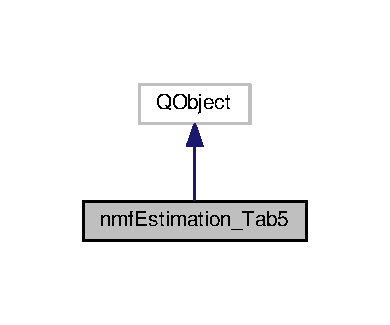
\includegraphics[width=187pt]{classnmf_estimation___tab5__inherit__graph}
\end{center}
\end{figure}


Collaboration diagram for nmf\+Estimation\+\_\+\+Tab5\+:\nopagebreak
\begin{figure}[H]
\begin{center}
\leavevmode
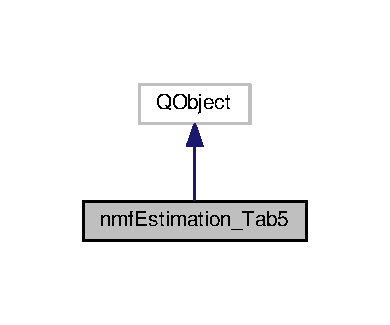
\includegraphics[width=187pt]{classnmf_estimation___tab5__coll__graph}
\end{center}
\end{figure}
\subsection*{Public Slots}
\begin{DoxyCompactItemize}
\item 
void {\bfseries callback\+\_\+\+Next\+PB} ()\hypertarget{classnmf_estimation___tab5_af379819acfabded6d10e0ae013468c49}{}\label{classnmf_estimation___tab5_af379819acfabded6d10e0ae013468c49}

\item 
void {\bfseries callback\+\_\+\+Prev\+PB} ()\hypertarget{classnmf_estimation___tab5_ad2dd05d2d965eeedc2faf2f476f183ba}{}\label{classnmf_estimation___tab5_ad2dd05d2d965eeedc2faf2f476f183ba}

\item 
void {\bfseries callback\+\_\+\+Load\+PB} ()\hypertarget{classnmf_estimation___tab5_ac4f696c9fc9816ce8c4aaab1c6d6248e}{}\label{classnmf_estimation___tab5_ac4f696c9fc9816ce8c4aaab1c6d6248e}

\item 
void {\bfseries callback\+\_\+\+Save\+PB} ()\hypertarget{classnmf_estimation___tab5_a916bfd238c215efec4592bdd122a9b25}{}\label{classnmf_estimation___tab5_a916bfd238c215efec4592bdd122a9b25}

\item 
void {\bfseries callback\+\_\+\+Set\+Algorithm} (Q\+String algorithm)\hypertarget{classnmf_estimation___tab5_aac14ac42066570e545a68596d056230b}{}\label{classnmf_estimation___tab5_aac14ac42066570e545a68596d056230b}

\item 
void {\bfseries callback\+\_\+\+Update\+Initial\+Observed\+Biomass} ()\hypertarget{classnmf_estimation___tab5_a040ea1a551c45f77d03bba8305cb9b49}{}\label{classnmf_estimation___tab5_a040ea1a551c45f77d03bba8305cb9b49}

\end{DoxyCompactItemize}
\subsection*{Signals}
\begin{DoxyCompactItemize}
\item 
void {\bfseries Reload\+Species} ()\hypertarget{classnmf_estimation___tab5_a294c657999cfbbcad8aec90b566a84f9}{}\label{classnmf_estimation___tab5_a294c657999cfbbcad8aec90b566a84f9}

\end{DoxyCompactItemize}
\subsection*{Public Member Functions}
\begin{DoxyCompactItemize}
\item 
\hyperlink{classnmf_estimation___tab5_a5b7a385222142f130e7f583b5fec6829}{nmf\+Estimation\+\_\+\+Tab5} (Q\+Tab\+Widget $\ast$tabs, nmf\+Logger $\ast$m\+\_\+logger, nmf\+Database $\ast$m\+\_\+database\+Ptr, std\+::string \&project\+Dir)
\begin{DoxyCompactList}\small\item\em \hyperlink{classnmf_estimation___tab5}{nmf\+Estimation\+\_\+\+Tab5} \+: class constructor \end{DoxyCompactList}\item 
void {\bfseries clear\+Widgets} ()\hypertarget{classnmf_estimation___tab5_acdcfaa4b4632eb18c1d322330e9b0adf}{}\label{classnmf_estimation___tab5_acdcfaa4b4632eb18c1d322330e9b0adf}

\item 
bool {\bfseries load\+Widgets} ()\hypertarget{classnmf_estimation___tab5_a520a89098cd0cbf3d5b2c65e2ad6f85c}{}\label{classnmf_estimation___tab5_a520a89098cd0cbf3d5b2c65e2ad6f85c}

\item 
bool {\bfseries load\+Widgets} (Q\+String Mohns\+Rho\+Label)\hypertarget{classnmf_estimation___tab5_a5ff9915bd9995191b8074c7ed8c9f00a}{}\label{classnmf_estimation___tab5_a5ff9915bd9995191b8074c7ed8c9f00a}

\item 
void {\bfseries read\+Settings} ()\hypertarget{classnmf_estimation___tab5_a0843bc4a49702394a0238fcd30184901}{}\label{classnmf_estimation___tab5_a0843bc4a49702394a0238fcd30184901}

\end{DoxyCompactItemize}


\subsection{Detailed Description}
Biomass Table. 

This table allows the user to enter and modify Observed Biomass data for each Species for every year in the year range. 

\subsection{Constructor \& Destructor Documentation}
\index{nmf\+Estimation\+\_\+\+Tab5@{nmf\+Estimation\+\_\+\+Tab5}!nmf\+Estimation\+\_\+\+Tab5@{nmf\+Estimation\+\_\+\+Tab5}}
\index{nmf\+Estimation\+\_\+\+Tab5@{nmf\+Estimation\+\_\+\+Tab5}!nmf\+Estimation\+\_\+\+Tab5@{nmf\+Estimation\+\_\+\+Tab5}}
\subsubsection[{\texorpdfstring{nmf\+Estimation\+\_\+\+Tab5(\+Q\+Tab\+Widget $\ast$tabs, nmf\+Logger $\ast$m\+\_\+logger, nmf\+Database $\ast$m\+\_\+database\+Ptr, std\+::string \&project\+Dir)}{nmfEstimation_Tab5(QTabWidget *tabs, nmfLogger *m_logger, nmfDatabase *m_databasePtr, std::string &projectDir)}}]{\setlength{\rightskip}{0pt plus 5cm}nmf\+Estimation\+\_\+\+Tab5\+::nmf\+Estimation\+\_\+\+Tab5 (
\begin{DoxyParamCaption}
\item[{Q\+Tab\+Widget $\ast$}]{tabs, }
\item[{nmf\+Logger $\ast$}]{m\+\_\+logger, }
\item[{nmf\+Database $\ast$}]{m\+\_\+database\+Ptr, }
\item[{std\+::string \&}]{project\+Dir}
\end{DoxyParamCaption}
)}\hypertarget{classnmf_estimation___tab5_a5b7a385222142f130e7f583b5fec6829}{}\label{classnmf_estimation___tab5_a5b7a385222142f130e7f583b5fec6829}


\hyperlink{classnmf_estimation___tab5}{nmf\+Estimation\+\_\+\+Tab5} \+: class constructor 


\begin{DoxyParams}{Parameters}
{\em tabs} & \+: the tab widget into which this Estimation tab will be placed \\
\hline
{\em logger} & \+: pointer to the application logger \\
\hline
{\em database\+Ptr} & \+: pointer to the application database \\
\hline
{\em project\+Dir} & \+: the project directory \\
\hline
\end{DoxyParams}


The documentation for this class was generated from the following files\+:\begin{DoxyCompactItemize}
\item 
nmf\+Estimation\+Tab05.\+h\item 
nmf\+Estimation\+Tab05.\+cpp\end{DoxyCompactItemize}

\hypertarget{classnmf_estimation___tab6}{}\section{nmf\+Estimation\+\_\+\+Tab6 Class Reference}
\label{classnmf_estimation___tab6}\index{nmf\+Estimation\+\_\+\+Tab6@{nmf\+Estimation\+\_\+\+Tab6}}


The Run Estimation Settings.  




{\ttfamily \#include $<$nmf\+Estimation\+Tab06.\+h$>$}



Inheritance diagram for nmf\+Estimation\+\_\+\+Tab6\+:\nopagebreak
\begin{figure}[H]
\begin{center}
\leavevmode
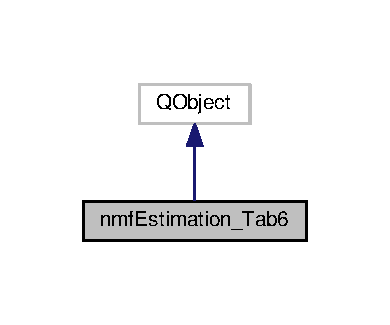
\includegraphics[width=187pt]{classnmf_estimation___tab6__inherit__graph}
\end{center}
\end{figure}


Collaboration diagram for nmf\+Estimation\+\_\+\+Tab6\+:\nopagebreak
\begin{figure}[H]
\begin{center}
\leavevmode
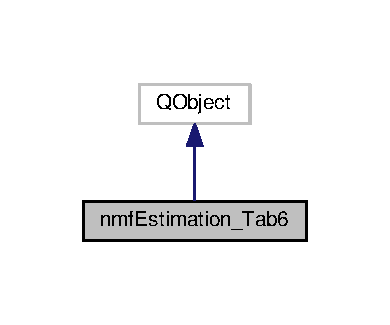
\includegraphics[width=187pt]{classnmf_estimation___tab6__coll__graph}
\end{center}
\end{figure}
\subsection*{Public Slots}
\begin{DoxyCompactItemize}
\item 
void {\bfseries callback\+\_\+\+Run\+PB} ()\hypertarget{classnmf_estimation___tab6_a3c5c8d50cc3593a54eb40c0c20fc585f}{}\label{classnmf_estimation___tab6_a3c5c8d50cc3593a54eb40c0c20fc585f}

\item 
void {\bfseries callback\+\_\+\+Load\+PB} ()\hypertarget{classnmf_estimation___tab6_ad8a9fc985e4a246cc57bbc1a0a30df77}{}\label{classnmf_estimation___tab6_ad8a9fc985e4a246cc57bbc1a0a30df77}

\item 
void {\bfseries callback\+\_\+\+Save\+PB} ()\hypertarget{classnmf_estimation___tab6_ab9d8966d571adcbf20eb563be2cee41f}{}\label{classnmf_estimation___tab6_ab9d8966d571adcbf20eb563be2cee41f}

\item 
void {\bfseries callback\+\_\+\+Prev\+PB} ()\hypertarget{classnmf_estimation___tab6_ad196ce3ba2a85c4184d2c2b53d011910}{}\label{classnmf_estimation___tab6_ad196ce3ba2a85c4184d2c2b53d011910}

\item 
void {\bfseries callback\+\_\+\+Estimation\+\_\+\+Tab6\+\_\+\+Font\+Size\+C\+MB} (Q\+String font\+Size)\hypertarget{classnmf_estimation___tab6_a58990cfc44584846cb25658883373cc7}{}\label{classnmf_estimation___tab6_a58990cfc44584846cb25658883373cc7}

\item 
void {\bfseries callback\+\_\+\+Estimation\+\_\+\+Tab6\+\_\+\+Mono\+CB} (int is\+Checked)\hypertarget{classnmf_estimation___tab6_af259a50d0e330514fbb7a5c1217c4877}{}\label{classnmf_estimation___tab6_af259a50d0e330514fbb7a5c1217c4877}

\item 
void {\bfseries callback\+\_\+\+Estimation\+\_\+\+Tab6\+\_\+\+Estimation\+Algorithm\+C\+MB} (Q\+String algorithm)\hypertarget{classnmf_estimation___tab6_a8b26cccc0e75bcc4fedba2b7ef4c3e20}{}\label{classnmf_estimation___tab6_a8b26cccc0e75bcc4fedba2b7ef4c3e20}

\item 
void {\bfseries callback\+\_\+\+Stop\+Val\+CB} (int is\+Checked)\hypertarget{classnmf_estimation___tab6_aeee2c7be131477d6efda0226dad88ab6}{}\label{classnmf_estimation___tab6_aeee2c7be131477d6efda0226dad88ab6}

\item 
void {\bfseries callback\+\_\+\+Stop\+After\+Time\+CB} (int is\+Checked)\hypertarget{classnmf_estimation___tab6_a598ae12325d506f449464de250bcb630}{}\label{classnmf_estimation___tab6_a598ae12325d506f449464de250bcb630}

\item 
void {\bfseries callback\+\_\+\+Stop\+After\+Iter\+CB} (int is\+Checked)\hypertarget{classnmf_estimation___tab6_ac6abc74e89aae1d73cd1d7c11cd89ace}{}\label{classnmf_estimation___tab6_ac6abc74e89aae1d73cd1d7c11cd89ace}

\item 
void {\bfseries callback\+\_\+\+Save\+Settings} ()\hypertarget{classnmf_estimation___tab6_a9397e07d0e936c72472ef817b9772155}{}\label{classnmf_estimation___tab6_a9397e07d0e936c72472ef817b9772155}

\end{DoxyCompactItemize}
\subsection*{Signals}
\begin{DoxyCompactItemize}
\item 
void {\bfseries Run\+Estimation} ()\hypertarget{classnmf_estimation___tab6_a5d492244aaf92c83b35fab7910874fd2}{}\label{classnmf_estimation___tab6_a5d492244aaf92c83b35fab7910874fd2}

\item 
void {\bfseries Show\+Run\+Message} (Q\+String msg)\hypertarget{classnmf_estimation___tab6_ad80fb4377497582c445bfe713e1d6c60}{}\label{classnmf_estimation___tab6_ad80fb4377497582c445bfe713e1d6c60}

\item 
void {\bfseries Set\+Algorithm} (Q\+String algorithm)\hypertarget{classnmf_estimation___tab6_a584d6f7ae74fa3decbc301db83fa3b14}{}\label{classnmf_estimation___tab6_a584d6f7ae74fa3decbc301db83fa3b14}

\item 
void {\bfseries Update\+Forecast\+Years} ()\hypertarget{classnmf_estimation___tab6_a3cde0546fa42f1e25fc48b5b01ec72ad}{}\label{classnmf_estimation___tab6_a3cde0546fa42f1e25fc48b5b01ec72ad}

\end{DoxyCompactItemize}
\subsection*{Public Member Functions}
\begin{DoxyCompactItemize}
\item 
\hyperlink{classnmf_estimation___tab6_a76d9d96d0040005c1beac82e6b1042e7}{nmf\+Estimation\+\_\+\+Tab6} (Q\+Tab\+Widget $\ast$tabs, nmf\+Logger $\ast$logger, nmf\+Database $\ast$database\+Ptr, std\+::string \&project\+Dir)
\begin{DoxyCompactList}\small\item\em \hyperlink{classnmf_estimation___tab6}{nmf\+Estimation\+\_\+\+Tab6} \+: class constructor \end{DoxyCompactList}\item 
void {\bfseries append\+Output\+TE} (Q\+String msg)\hypertarget{classnmf_estimation___tab6_a81688b028744e43740ee3ceb19ffe99a}{}\label{classnmf_estimation___tab6_a81688b028744e43740ee3ceb19ffe99a}

\item 
void {\bfseries clear\+Output\+TE} ()\hypertarget{classnmf_estimation___tab6_aff1da981b2dcc93776be29bba7ec4cb1}{}\label{classnmf_estimation___tab6_aff1da981b2dcc93776be29bba7ec4cb1}

\item 
Q\+String {\bfseries get\+Data\+Path} ()\hypertarget{classnmf_estimation___tab6_acad2efbd876dc189511de13ad8829166}{}\label{classnmf_estimation___tab6_acad2efbd876dc189511de13ad8829166}

\item 
std\+::string {\bfseries get\+Current\+Algorithm} ()\hypertarget{classnmf_estimation___tab6_a81c9d5fa7c08230396d99728f24b23a9}{}\label{classnmf_estimation___tab6_a81c9d5fa7c08230396d99728f24b23a9}

\item 
std\+::string {\bfseries get\+Current\+Minimizer} ()\hypertarget{classnmf_estimation___tab6_aff516e5c4af59ec185d38533d99fcc3b}{}\label{classnmf_estimation___tab6_aff516e5c4af59ec185d38533d99fcc3b}

\item 
std\+::string {\bfseries get\+Current\+Objective\+Criterion} ()\hypertarget{classnmf_estimation___tab6_ac75d359d6f19639d57d49fe09891d920}{}\label{classnmf_estimation___tab6_ac75d359d6f19639d57d49fe09891d920}

\item 
bool {\bfseries load\+Widgets} ()\hypertarget{classnmf_estimation___tab6_aa491ce6e38d28a78bd96ec8d10df4f13}{}\label{classnmf_estimation___tab6_aa491ce6e38d28a78bd96ec8d10df4f13}

\item 
void {\bfseries read\+Settings} ()\hypertarget{classnmf_estimation___tab6_aa851675904001978da6ce35298bf3012}{}\label{classnmf_estimation___tab6_aa851675904001978da6ce35298bf3012}

\item 
void {\bfseries refresh\+Msg} (Q\+Font font, Q\+String msg)\hypertarget{classnmf_estimation___tab6_a9d7c76dd70b2fc9a36beaaa4a4fb36d9}{}\label{classnmf_estimation___tab6_a9d7c76dd70b2fc9a36beaaa4a4fb36d9}

\item 
void {\bfseries save\+Settings} ()\hypertarget{classnmf_estimation___tab6_a7ad46555e85c23ffb9cc84c5446ffae9}{}\label{classnmf_estimation___tab6_a7ad46555e85c23ffb9cc84c5446ffae9}

\item 
bool {\bfseries save\+Settings\+Configuration} (bool verbose, std\+::string current\+Settings\+Name)\hypertarget{classnmf_estimation___tab6_ad8d3bd503e684ef029d1afc1040d36b5}{}\label{classnmf_estimation___tab6_ad8d3bd503e684ef029d1afc1040d36b5}

\item 
void {\bfseries save\+System} (bool Run\+Checks)\hypertarget{classnmf_estimation___tab6_a94d15864888d0148cc11b18c99a1a3bf}{}\label{classnmf_estimation___tab6_a94d15864888d0148cc11b18c99a1a3bf}

\item 
void {\bfseries set\+Font} (Q\+Font font)\hypertarget{classnmf_estimation___tab6_aec4866528626ed36cd4c393f94603247}{}\label{classnmf_estimation___tab6_aec4866528626ed36cd4c393f94603247}

\item 
void {\bfseries set\+Output\+TE} (Q\+String msg)\hypertarget{classnmf_estimation___tab6_afd007d6605c7b3d57b32f4c33ab82ced}{}\label{classnmf_estimation___tab6_afd007d6605c7b3d57b32f4c33ab82ced}

\end{DoxyCompactItemize}


\subsection{Detailed Description}
The Run Estimation Settings. 

These widgets allow the user to enter and save the parameters required to run an Estimation. There\textquotesingle{}s also a text widget which shows a summary to the user of what transpired after the user hits the Run button. 

\subsection{Constructor \& Destructor Documentation}
\index{nmf\+Estimation\+\_\+\+Tab6@{nmf\+Estimation\+\_\+\+Tab6}!nmf\+Estimation\+\_\+\+Tab6@{nmf\+Estimation\+\_\+\+Tab6}}
\index{nmf\+Estimation\+\_\+\+Tab6@{nmf\+Estimation\+\_\+\+Tab6}!nmf\+Estimation\+\_\+\+Tab6@{nmf\+Estimation\+\_\+\+Tab6}}
\subsubsection[{\texorpdfstring{nmf\+Estimation\+\_\+\+Tab6(\+Q\+Tab\+Widget $\ast$tabs, nmf\+Logger $\ast$logger, nmf\+Database $\ast$database\+Ptr, std\+::string \&project\+Dir)}{nmfEstimation_Tab6(QTabWidget *tabs, nmfLogger *logger, nmfDatabase *databasePtr, std::string &projectDir)}}]{\setlength{\rightskip}{0pt plus 5cm}nmf\+Estimation\+\_\+\+Tab6\+::nmf\+Estimation\+\_\+\+Tab6 (
\begin{DoxyParamCaption}
\item[{Q\+Tab\+Widget $\ast$}]{tabs, }
\item[{nmf\+Logger $\ast$}]{logger, }
\item[{nmf\+Database $\ast$}]{database\+Ptr, }
\item[{std\+::string \&}]{project\+Dir}
\end{DoxyParamCaption}
)}\hypertarget{classnmf_estimation___tab6_a76d9d96d0040005c1beac82e6b1042e7}{}\label{classnmf_estimation___tab6_a76d9d96d0040005c1beac82e6b1042e7}


\hyperlink{classnmf_estimation___tab6}{nmf\+Estimation\+\_\+\+Tab6} \+: class constructor 


\begin{DoxyParams}{Parameters}
{\em tabs} & \+: the tab widget into which this Estimation tab will be placed \\
\hline
{\em logger} & \+: pointer to the application logger \\
\hline
{\em database\+Ptr} & \+: pointer to the application database \\
\hline
{\em project\+Dir} & \+: the project directory \\
\hline
\end{DoxyParams}


The documentation for this class was generated from the following files\+:\begin{DoxyCompactItemize}
\item 
nmf\+Estimation\+Tab06.\+h\item 
nmf\+Estimation\+Tab06.\+cpp\end{DoxyCompactItemize}

%--- End generated contents ---

% Index
\backmatter
\newpage
\phantomsection
\clearemptydoublepage
\addcontentsline{toc}{chapter}{Index}
\printindex

\end{document}
